\chapter{Preliminaries:\\ Building Blocks of WSN} \label{Chp: Building Blocks}

In this chapter, we introduce the building blocks of a WSN using OSI model\cite{OSI}.

The data channel in OSI model is descried as a set of protocols stacked layer by layer from the Physical Layer at the bottom to the Application Layer at the top (\Cref{fig: OSI model}). Ideally, lower layer protocols provide an universal  interface to upper layer protocols; thus providing flexibility to protocol choice in different scenarios as well as interoperability between nodes with different lower level structures.

\begin{figure*}[h!]
	\centering
	{
		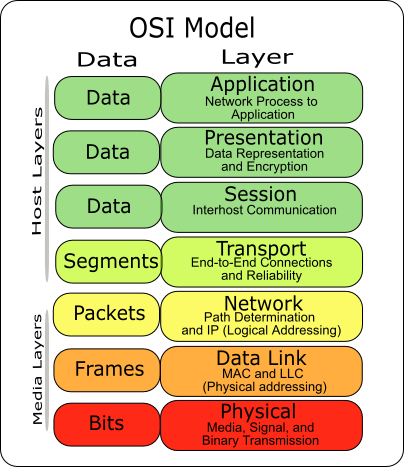
\includegraphics[width=0.4\textwidth,]{fig/Osi-model-jb.png}
	}
	\caption{OSI model} \label{fig: OSI model}
\end{figure*}

\Cref{fig: OSI channel} demonstrates a typical data transmission in OSI modelled network. The application data is encapsulated by the sender from top to the bottom, with each encapsulation adds additional metadata, namely protocol headers, to the data. The receiver unwinds the process and reads out the data.

\begin{figure*}[h!]
	\centering
	{
		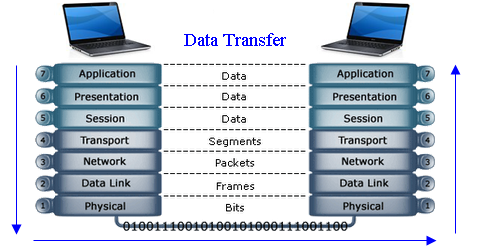
\includegraphics[width=0.6\textwidth,]{fig/osi-model.png}
	}
	\caption{Data Transfer in OSI model} \label{fig: OSI channel}
\end{figure*}

However, in real world scenarios the boundaries between the top three layers are usually ambiguous; many context, including this report, simply refers them all together as Application Layer. In most scenarios the application only needs the Transport Layer interfaces and anything beneath is transparent.

A selection of protocols at each layer is called a protocol suite, or a protocol stack. 8 bits is called an OCTET in network terminology but for readability in general computer science we use BYTE to represent the unit of 8 bits.

Protocols from Physical Layer to Transport Layer are implemented by hardware or kernel. Since most IoT devices are extremely resource constrained; thus it is hard to directly transplant the widely used TCP/IP protocol suite to WSNs. Instead, different protocols and operating systems are specifically designed for WSN applications. Contiki\cite{Contiki} is a highly customisable IoT system with 6LoWPAN\cite{rfc4919} support and can run on many recent IoT hardware, OpenWSN\cite{OpenWSN} is also a popular IoT system that has well integrated 6LoWPAN with CoAP\cite{rfc7252} and FreeRTOS\cite{FreeRTOS} is optimised for real time applications, etc. There are many other IoT systems and protocols that we do not list here. In this research, we build our experimental WSN over Contiki with 6LoWPAN due to their popularity in academic and industry.

Following in \Cref{Chp: Building Blocks} we introduce the building blocks of our experimental WSN from the bottom to the top in OSI model.

\section{Physical Layer}
Physical Layer protocols (or standards) specify the hardware requirements. They basically defines how a bit is transmitted over a physical medium.

WSN features, as can be seen by its name, wireless connectivity. 802.15.4\cite{802154} standard is supported in many recent WSN devices. The  802.15.4 Physical Layer specification, 802.15.4 PHY, is crafted to be suitable for embedded wireless devices emphasising low energy, low cost and low speed. Bluetooth Low Energy\cite{BLE}, BLE, is another candidate for WSN with similar features. \cite{802154BLE} provides a performance analysis of 802.15.4 and BLE.

\Cref{Fig: 802.15.4 PHY Frame} shows the constitution of a Physical Layer frame. A frame is a bit string transmitted sequentially from the left in the figure to the right. We use the same representations for the rest in \Cref{Chp: Building Blocks}.

\begin{table}[h!]
	\centering
	\begin{tabular}{|c|c|c|c|c|}
		\hline
		Preamble & SFD & MAC Frame Length & Reserved & MAC Frame\\ \hline
	\end{tabular}
	\caption{802.15.4 PHY Frame}
	\label{Fig: 802.15.4 PHY Frame}
\end{table}

We omit the further details of 802.15.4 PHY standard as they strongly relate to hardware details which is beyond the scope of this report. We give only a brief explanation of the contents in the frame.

\textbf{Preamble} is a flag used for hardware synchronisation. \textbf{Start Frame Delimiter}, SFD, is a constantly 0xE5 for 802.15.4 frames which marks the begin of data in this frame. \textbf{MAC Frame Length} is a value of 0 to 127 indicating the number of bytes in the following \textbf{MAC Frame}, which we explain in \Cref{Sec: Data Link Layer}.

Our experimental WSN is built on TelosB\cite{TelosB} and CC2538\cite{CC2538}. Wismote\cite{Wismote} is also used in Cooja simulations.

\section{Data Link Layer} \label{Sec: Data Link Layer}
Data Link Layer protocols manages the Physical Layer channel. In case of WSN, this is effectively Radio Frequency, RF. Data Link protocols are strongly related to physical features of underlining devices. 

Data Link Layer is  also referred as Media Access Control, MAC, Layer for convenience. A MAC Frame is the atomic data transferring unit in this layer. MAC Layer protocols define data transmission between physically connected devices, i.e. single hop communication. Packet forward is defined in upper layer protocols.

In case of WSN, a MAC Frame is always broadcasted to the sender’s neighbour due to the physical nature of RF. To avoid interference, MAC protocols adopts  techniques such as CSMA/CA \cite{802154} or TSCH\cite{TSCH} to solve the problem of how MAC Frames should be sent. Further more, other techniques like ContikiMAC\cite{ContikiMAC} proposes a sub Radio Duty Cycle, RDC, Layer protocol that aims to improve the energy efficiency of RF.

As of this research, we are more focused on the contents in a MAC Frame defined by 802.15.4 MAC Layer specification\cite{802154}, 802.15.4 MAC.

\subsection{802.15.4 MAC} \label{Subsec: 802.15.4 MAC}
802.15.4 MAC defined four types of MAC Frames.
\begin{description}[style=nextline]
	\item[\textbf{Beacon}] 
	Beacon frame is broadcasted to physically organise the network.
	\item[\textbf{Command}] 
	Command frame is used for data channel maintenance.
	\item[\textbf{Data}] 
	Data frame carries data from upper layer protocols.
	\item[\textbf{ACK}] 
	ACK frame only optionally sent in response when requested by other frames to notify the sender that the frame is received. Some protocols use ACK frames, e.g. ContikiMAC uses it to inform the sender that the frame is received and hence terminates the resending process of sender.
\end{description}

We are particularly interested in Data frames as they are most relevant to application data. \Cref{Fig: 802154 Data Frame} describes its format.

\begin{figure*}[h!]
	\centering
	\begin{tabular}{|c|c|c|c|c|}
		\multicolumn{3}{c}{\textit{MAC Header}}                           & \multicolumn{1}{c}{\textit{MAC Payload}} & \multicolumn{1}{c}{\textit{MAC Footer}}     \\ \hline
		2 (bytes)     & 1                    & 4 to 20              & *           & 2              \\ \hline
		Frame Control & Sequence Number & Address Information & Data        & Frame Checksum \\ \hline
	\end{tabular}
	\caption{802.15.4 Data Frame}
	\label{Fig: 802154 Data Frame}
\end{figure*}

\begin{description}[style=nextline]
	\item[\textbf{Frame Control}]
	This field contains the bit flags instructing how the receiver should interpret this frame, such as the type of frame, with ACK and security options on or not, and format of addresses, etc. When the security option is enabled, additional field will be added to the frame. We explain the security enabled frame later in \Cref{Subsec: 802154 Sec}. The full details of flags is defined by \cite{802154}.
	
	\item[\textbf{Sequence Number}]
	The sequence number is increased by one for each MAC Frame sent and wraps to 0 when reached maximum. The sequence number is mostly used to match ACKs when requested.
	
	\item[\textbf{Address Information}]
	This field contains source and destination MAC address of this frame. Their length are variable and is specified in Frame Control. Simply speaking, longer addresses are for larger networks and shorter for smaller ones. MAC address is derived from hardware and should be unique but configurable during runtime. As stated earlier, a MAC Frame is always received by all neighbours of the sender; therefore the receiver who does not match the destination will immediately drop the frame without processing it to upper layer.
	
	\item[\textbf{Data}]
	This is the MAC Layer data containing upper layer protocol headers and application data.
	
	\item[\textbf{Frame Checksum}]
	The checksum is used to check and correct the error induced by physical channel.
\end{description}

Frame Control, Sequence Number and Address Information together are called MAC Header. Data is therefore called MAC Payload respectively. 

As specified in 802.15.4 PHY, Maximum Transmission Unit, MTU, required by 802.15.4 MAC Frame is 127 bytes including the MAC header and footer. In other words, 802.15.4 compatible hardware are guaranteed to send frames up to 127 bytes but frames exceeding this value might be silently discarded. Since MAC Header and Footer consumes 25 bytes in a Data frame, there is actually 102 bytes left for MAC Payload.

Setting the security flag in Frame Control enables 802.15.4 Security and adds additional fields into the MAC header, which we describe in \Cref{Subsec: 802154 Sec}.

\subsection{802.15.4 Security} \label{Subsec: 802154 Sec}
802.15.4 Security is based on Authenticated Encryption with Associated Data, AEAD, with AES-128 being the underlining block cipher. Specifically, it provides encryption for MAC Payload and authenticity for the whole MAC Frame.

The format of a 802.15.4 Data frame with security option set is described in \Cref{Fig: 802154 sec frame}.

\begin{figure*}[h!]
	\centering
	\begin{tabular}{|c|c|c|c|c|c|c|}
		\multicolumn{4}{c}{\textit{MAC Header}}                                                             & \multicolumn{2}{c}{\textit{MAC Payload}} & \multicolumn{1}{c}{\textit{MAC Footer}}     \\ \hline
		\multicolumn{3}{|c|}{\multirow{2}{*}{As MAC Header in \Cref{Fig: 802154 Data Frame}}} & 0 to 14 (bytes)                    & *             & 0/4/8/16         & 2              \\ \cline{4-7} 
		\multicolumn{3}{|c|}{}                                           & Auxiliary Security Header & Data          & MIC              & Frame Checksum \\ \hline
	\end{tabular}
	\caption{802.15.4 Frame with security option enabled} \label{Fig: 802154 sec frame}
\end{figure*}

The Auxiliary Security Header controls the security primitive and materials in 802.15.4 Security as shown in \Cref{Fig: Auxiliary Security Header of 802.15.4 Security}.

\begin{figure*}[h!]
	\center
	\begin{tabular}{|c|c|c|}
	\hline
	\multicolumn{3}{|c|}{Auxililary Security Header} \\ \hline
	3 bits          & 4 byte         & *             \\ \hline
	Security Level  & Frame Counter  & Key Strategy  \\ \hline
	\end{tabular}
	\caption{Auxiliary Security Header of 802.15.4 Security}
	\label{Fig: Auxiliary Security Header of 802.15.4 Security}
\end{figure*}

\begin{description}[style=nextline]
	\item[\textbf{Security Level}]
	Security Level is represented by the first 3 bits in Auxiliary Security Header. The highest bit enables encryption and lower two bits controls the length of Message Integrity Code, MIC, which is equivalent to Message Authenticate Code in cryptographic terms.  MIC of $0$ length indicates no authentication. Particularly, the security level can be configured to be:
	\begin{itemize}
		\item Encryption only. Only MAC Payload is encrypted in CTR mode.
		\item Authentication only. A CBC-MIC\footnote{Equivalent to CBC-MAC in cryptographic term.} computed on the whole frame is attached to the end of Data. Data is transmitted in plaintext. Length of the MIC can be either 32, 64 or 128 bits based on the lower two bits of Security Level.
		\item Encryption and authentication. The whole frame is processed in CCM*\cite{802154} mode. MAC Header is the associated data and MAC Payload the plaintext. The asterisk symbol requires that the nonce, or IV, must can be decoded to uniquely determine the exact format of output ciphertext. Length of the MIC can be either 32, 64 or 128 bits based on the lower two bits of Security Level.
	\end{itemize}
	\item[\textbf{Frame Counter}]
	4 bytes of Auxiliary Security Header is occupied by Frame Counter which increases by one for each frame sent. It constitutes part of the nonce in CCM* mode and is also used for replay detection.
	\item[\textbf{Key Strategy}]
	Key Strategy instructs which key to be used for this frame. The keys are presumed to be pre-shared in PAN\footnote{Personal Area Network} Information Base, PIB, which is a database containing information that is shared among the network. Keys are managed by groups and indexes within a group. The definition of groups depends on upper layer applications. The length of Key Strategy is variable.
\end{description}

More details of Auxiliary Security Header is defined by \cite{802154}.

Access Control List, ACL, is a data structure used to manage the keys during runtime. Each entry of ACL is paired with another node.  An ACL entry contains the following elements:
\begin{description}[style=nextline]
	\item[\textbf{Address}]
	The remote address, used as an identifier of ACL entry.
	\item[\textbf{Security Suite}]
	Effectively the Security Level associated to the remote address.
	\item[\textbf{Key}]
	The paired cryptographic key associated to the remote address.
	\item[\textbf{Last Initial Vector}]
	Nonce used for the last outgoing frame. Used to deduce next nonce to use.
	\item[\textbf{Replay Counter}]
	Nonce received for the last incoming frame. Used when replay protection is on.
\end{description}

One thing to be noticed is that neither Key Strategy nor ACL is implemented on our platform. We give more details about key management of 802.15.4 Security in Contiki implementation in \Cref{Subsec: 802.15.4 Security Implementation in Contiki}.

\subsection{Nonce of CCM* in 802.15.4 Security}
As stated earlier in \Cref{Subsec: 802154 Sec}, CCM* requires that the format of ciphertext can be uniquely deduced from the nonce. \Cref{Fig: CCM nonce} describes the nonce used for encryption.

\begin{figure*}[h!]
	\centering
	\begin{tabular}{|c|c|c|c|c|}
		\hline 
		1 (bytes) & 8              & 4             & 1              & 2             \\ \hline
		Flag      & Source Address & Frame Counter & Security Level & Block Counter \\ \hline
	\end{tabular}
	\caption{CCM* nonce for encryption}
	\label{Fig: CCM nonce}
\end{figure*}

\begin{description}[style=nextline]
	\item[\textbf{Flag}]
	 Deduced by MTU. In case of 802.15.4, it is constantly 0x02.
	\item[\textbf{Source Address}]
	Address of sender. Addresses less than 8 bytes will be extended.
	\item[\textbf{Frame Counter}]
	Directly mapped from Frame Counter in Auxiliary Security Header.
	\item[\textbf{Security Level}]
	Directly mapped from Security Level in Auxiliary Security Header with the highest bit set to $0$. Security Level solely determines the format of ciphertext.
	\item[\textbf{Block Counter}]
	Index of data blocks in MAC payload, with the first block being 0 and increases by one for each block. The block length is 128 bits since AES-128 is the underlining block cipher.
\end{description}

802.15.4 Security could either be implemented by hardware and/or software. Some platform may not support the security option, or only a sub set. We describe the 802.15.4 Security implementation on Contiki in \Cref{Subsec: 802.15.4 Security Implementation in Contiki}.

\subsection{802.15.4 Security Implementation in Contiki} \label{Subsec: 802.15.4 Security Implementation in Contiki}
noncoresec\cite{noncoresec} is the 802.15.4 Security implementation in Contiki. It is a reduced implementation of 802.15.4 Security which supports only a network shared key hard coded into the kernel code.

\subsection{Sub Layer: RDC Layer}

In practical, the radio transceiver turned out to be the most energy consuming part in a sensor node. Further more, listening to data consumes more energy than sending. Therefore an improvement of energy efficiency is to switch off the transceiver for most of the time and only turn it on when there is data on air. The Radio Duty Cycle, RDC, Sub Layer is therefore defined as part of MAC Layer which controls the behaviour of radio transceiver.

There are two RDC protocols implemented in our platform.

\begin{itemize}
\item \textbf{nullrdc}. There is no RDC protocol. The transceiver is always kept on.
\item \textbf{ContikiMAC\cite{ContikiMAC}}. The transceiver is kept off for most of the time and only wakes up for a short period. If data transmission is detected during the wake-up period, the receiver keeps the transceiver on until the frame is received and informs the sender with an ACK. On the other hand, the sender continuously retransmits the frame until an ACK is received or timeout.
\end{itemize}

Time-Slotted Channel Hopping\cite{TSCH}, TSCH, is another RDC protocol that is adopted by OpenWSN. We omit its further detail as it is not yet implemented on our platform.

\section{Network Layer} \label{Sec: Network Layer}
The MAC Layer protocols defined the data transmission over directly linked nodes. However, real world applications are usually deployed in a wider range that physically cannot be covered by only direct connections, such as smart city applications. The solution is to build a logical connection that allows the data to be forwarded by intermediate nodes until it reaches the destination. Such logical connection is called a multi hop connection with respect to directly connected single hop connection. As a result, arbitrary nodes can connect to each others and hence forms a network.

Network Layer protocols aim at the routing and addressing problems. The transmission unit in Network Layer is called a packet. The headers and payload constitutes the MAC Payload as in \Cref{Fig: 802154 Data Frame}.

There are two typical types of network in WSN applications:
\begin{description}[style=nextline]
	\item[\textbf{Star Network}]
	Star network is a type of centralised network as depicted in \Cref{fig: Star Network}. Each node is directly linked to the centre one. 
	\item[\textbf{Mesh Network}]
	Mesh network has a decentralised structure as depicted in \Cref{fig: Mesh Network}. Comparing to star network, packets are routed in a mesh network.
\end{description}
%CONTINUE FROM HERE 20160218
\begin{figure*}
	\centering
	\begin{subfigure}[b]{0.5\textwidth}
		{
			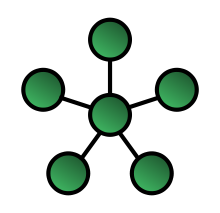
\includegraphics[width=0.5\textwidth,]{fig/StarNetwork.png}
		}
		\subcaption{Star Network} \label{fig: Star Network}
	\end{subfigure}
	\begin{subfigure}[b]{0.5\textwidth}
		{
			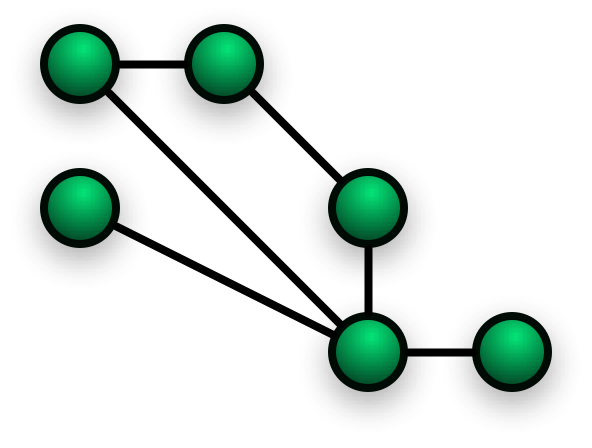
\includegraphics[width=0.5\textwidth,]{fig/NetworkTopology-Mesh.png}
		}
		\subcaption{Mesh Network} \label{fig: Mesh Network}
	\end{subfigure}
	\caption{Network Topologies} \label{fig: Network topologies}
\end{figure*}

%Some network are built with a hybrid approach of star network and mesh network, e.g. the Cluster Tree Network of Zigbee\cite{Zigbee} as showed in \Cref{fig: ZigBee Topologies}.
%
%\begin{figure*}[h!]
%	\centering
%	{
%		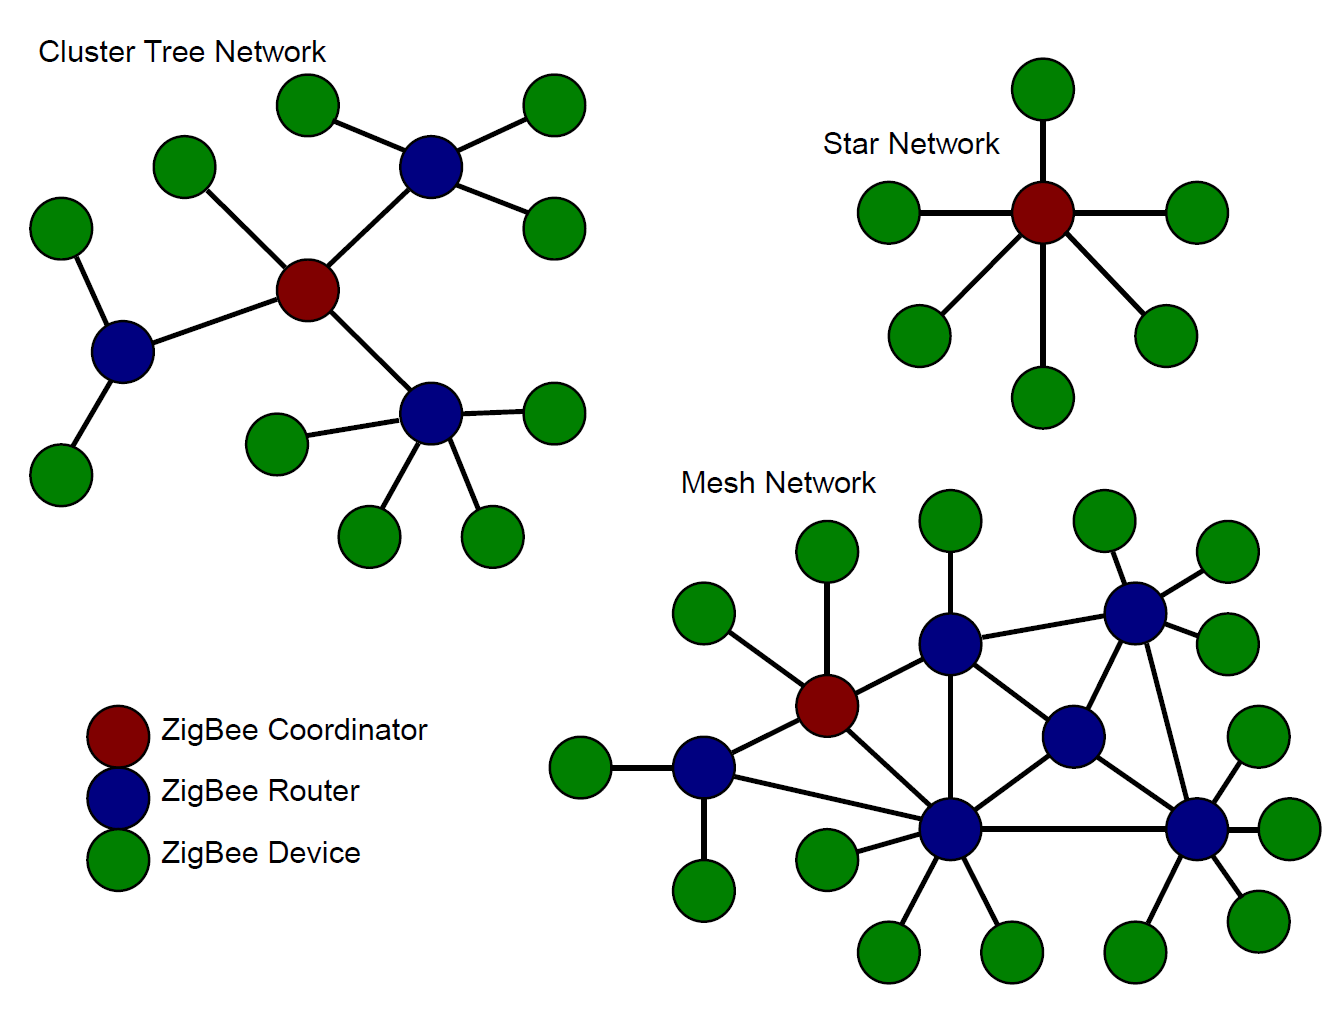
\includegraphics[width=0.7\textwidth,]{fig/ZigBeeTopologies.png}
%	}
%	\caption{Different ZigBee Network Topologies} \label{fig: ZigBee Topologies}
%\end{figure*}

Star network is easier to implement and therefore requires less resources. Mesh network is more complicated but it is more flexible, scalable and robust.

In this research, we build our experimental WSN using 6LoWPAN without loss of generality, as it is supported by most recent WSN systems.



\subsection{6LoWPAN} \label{Subsec: 6LoWPAN}
6LoWPAN is an emerging standard in WSN applications. 6LoWPAN has the following features: 
\begin{itemize}
	\item It is standardised by IETF and is well supported in industry.
	\item Each device is assigned an IPv6 address. This feature provides a great potential of interoperability with other Internet devices, such as a desktop or a smart phone.
	\item As a mesh network, it is flexible, scalable and robust, since the network can dynamically reorganise itself during runtime.
\end{itemize}

Simply speaking , 6LoWPAN packets can be categorised into two classes:
\begin{itemize}
	\item \textbf{IPv6 Data Packets}
	\item \textbf{ICMPv6 Packets}
\end{itemize}
We give a brief explanation of their contents in \Cref{Subsec: IPv6 Data Packets} and \Cref{Subsec: ICMPv6} respectively.

\subsection{6LoWPAN Adaptation Sub Layer} \label{Subsec:6LoWPAN Adaptation Sub Layer}
A sub layer is defined in 6LoWPAN standard\cite{rfc4944} which adapts IPv6\cite{rfc2460} to constrained environment by header compression. An adaption headers is prepended before the IPv6 header as shown in \Cref{Fig: 6LoWPAN Adaptation Header}. 

\begin{figure*}[h!]
	\centering
	\begin{tabular}{|l|l|l|}
		\hline
		6LoWPAN Adaptation Header & Compressed IPv6 Header & IPv6 Payload \\ \hline
	\end{tabular}
	\caption{6LoWPAN Adaptation Header}
\label{Fig: 6LoWPAN Adaptation Header}
\end{figure*}

The compression is basically done by:
\begin{itemize}
	\item Optimised encoding. Take the Hop Limit, HLIM or TTL (Time To Live), field for example, the frequently used values, 1, 64 and 255, are represented in 2 bits as 01b, 10b and 11b respectively, saving 6 bits from its original 1 byte field.
	\item Shortened addresses. Since 6LoWPAN has usually less devices than a normal IPv6 network, the unused higher bits can be omitted. The shortened addresses can be extended on need.
\end{itemize}

The header compression is lossless; thus an equivalent IPv6 header can always be reconstructed. We omit further details of compression as it is beyond the scope of this research but the scheme is defined in \cite{rfc6282}.

In addition to header compression information, 6LoWPAN Adaptation sub layer may optionally contains packet fragmentation information and routing information. We omit further details of them as they are beyond the scope of this research. Details are defined in \cite{rfc4944}.

\subsection{IPv6 Data Packets} \label{Subsec: IPv6 Data Packets}

IPv6 Data Packets carry the IPv6 Payload. In 6LoWPAN, the IPv6 header is compressed as described in \Cref{Subsec:6LoWPAN Adaptation Sub Layer}. In this section, we use a standard IPv6 header in description instead for convenience, as it is bijective to its compressed format.

IPv6 packet is defined in \cite{rfc2460}. We show its basic format in \Cref{Fig: Basic IPv6 Packet Format}. Length information are omitted in the figure as they are inconsistent when compressed.

\begin{figure*}[h!]
\center
	\begin{tabular}{l|c|c|c|c|c|c|}
	\cline{2-7}
	\multirow{2}{*}{\textit{IP Header}} & Version & Traffic Class & Flow Label & Payload Length & Next Header & Hop Limit \\ \cline{2-7} 
	                                & \multicolumn{3}{c|}{Source Address}  & \multicolumn{3}{c|}{Destination Address} \\ \cline{2-7} 
	\textit{IP Payload}                 & \multicolumn{6}{c|}{Payload}                                                    \\ \cline{2-7} 
	\end{tabular}
	\caption{Basic IPv6 Packet Format} \label{Fig: Basic IPv6 Packet Format}
\end{figure*}

\begin{description}[style=nextline]
	\item[\textbf{Version}]
	In 6LoWPAN this is constant 0x6.
	\item[\textbf{Traffic Class}]
	This field is default by 0 and may be set by an upper layer application as a hint of packet. A router can act accordingly to this field, such as adjusting the priority of packet, or even modify this value upon forward. The support for values other than $0$ is optional.
	\item[\textbf{Flow Label}]
	This field is intended to label a logical data path at Network Layer. The IPv6 standard\cite{rfc2460} states  it should ``be used by a source to label sequences of packets for which it requests special handling by the IPv6 routers, such as non-default quality of service or `real-time` service``. Support to this field is optional.
	\item[\textbf{Payload Length}]
	This field specifies the length of Payload.
	\item[\textbf{Next Header}]
	This field specifies the Transportation Layer protocol to be used. In WSN applications this is usually UDP. We introduce more details in \Cref{Sec: Transport Layer}.
	\item[\textbf{Hop Limit}]
	Hop Limit, HLIM, also known as Time To Live, TTL. It decreases by one whenever the packet is forwarded. The packet will be dropped when this value reaches $0$. This prevents a packet from being infinitely forwarded.
	\item[\textbf{Source Address and Destination Address}]
	These are the IPv6 addresses of sender and receiver. These fields are normally consistent during routing of a packet. In comparison, source and destination in MAC Frame varies on each hop, as an intermediate receiver becomes the sender of next hop.
	\item[\textbf{Payload}]
	This field contains the upper layer protocol headers and application data.
\end{description}

One thing to be noticed is that Traffic Class and Flow Label is not yet fully defined by IPv6 standard\cite{rfc2460}. 

Extension headers are also defined in IPv6\cite{rfc2460}, including IPsec and fragmentation ,etc. These headers are optional and are chained by Next Header.

\begin{description}[style=nextline]
\item[\textbf{IPsec}]
Overview of IPsec is defined in \cite{rfc4301}. The Authentication Header, AH, is defined by \cite{rfc4302} and Encapsulating Security Payload, ESP, defined by \cite{rfc4303}. AH authenticates all IP Headers (basic IPv6 header in \Cref{Fig: Basic IPv6 Packet Format} plus the extensions), except fields those might be modified by a router such as HLIM. ESP provides encryption over IP Payload. Enabling IPsec over IPv6 adds 40 bytes to the IP Header which is unacceptable in constrained environment. \cite{6LoWPANIPsec} and \cite{CompressIPsec} discusses compression of IPsec over 6LoWPAN. \cite{ContikiIPsec} describes an implementation of IPsec over Contiki but it is not yet adopted by the latest released Contiki 3.0.
\end{description}

We omit further details of other extension headers as they are mostly used to handle routing and fragmentation and thus beyond the scope of this report.

\subsection{ICMPv6 Packets} \label{Subsec: ICMPv6}
Internet Control Message Protocol for IPv6, ICMPv6, is a set of messages that are used to maintain the network. \cite{rfc4443} defines the general format. 

%IPv6 General Format
In IPv6, an ICMP messages is preceded by an IPv6 Basic Header and optional IPv6 extension headers with the last Next Header field set to ICMP as in \Cref{Fig: ICMP with IPv6}. The IP Payload in \Cref{Fig: Basic IPv6 Packet Format} is replaced by an ICMP message in this case.

\begin{figure*}[h!]
	\centering
	\begin{tabular}{|l|l|l|}
		\hline
		IPv6 Basic Header & Extension Headers (optional) & ICMP Message \\ \hline
	\end{tabular}
	\caption{ICMP Message with IPv6 Headers}
	\label{Fig: ICMP with IPv6}
\end{figure*}

The general format of an IPv6 message is described in \cite{rfc4443} as \Cref{Fig: General Format of ICMPv6 Message}.
\begin{figure*}[h!]
	\centering
	\begin{tabular}{|c|c|c|c|}
	\hline
	1 (byte) & 1    & 2        & *            \\ \hline
	Type     & Code & Checksum & Message Body \\ \hline
	\end{tabular}
	\caption{General Format of ICMPv6 Message}
	\label{Fig: General Format of ICMPv6 Message}
\end{figure*}

\begin{description}[style=nextline]
\item[\textbf{Type}]
There are two groups of types of messages defined in \cite{rfc4443}. Error message has a Type value in $[0,127]$ which indicates an error in the network. Information messages has a type value in $[128,255]$ which provide management information to nodes in the network.
\item[\textbf{Code}]
Each type of ICMP message defines its own code to indicate the further details.
\item[\textbf{Checksum}]
Checksum for the packet.
\item[\textbf{Message Body}]
Message Body varies according to Type and Code.
\end{description}
Full details are defined by \cite{rfc4443},

We explain only a minor set of ICMP Messages that we have successfully observed in our experimental WSN.
%Error messages, informative message
\begin{description}[style=nextline]
	\item[\textbf{Echo Request and Reply Messages}]
	These are diagnostic ICMP Information messages. Upon receiving an ICMP Echo Request, the receiving node is required by \cite{rfc4443} to reply with an identical ICMP message except the source and destination addresses are inverted. The Echo Request is typically sent by a PING command for diagnostic reasons such as testing of connectivity or measuring the Round Trip Time, RTT, of a data path. The response of ICMP Echo is enabled in Contiki by default but it is disabled on many Internet server for security reasons. These packets are also commonly known as PING packets.
	
	\item[\textbf{RPL Messages}]
	A family of ICMPv6 messages, RPL Messages, are defined by \cite{rfc6550}. RPL Messages are fundamental in foundation and self-organisation a 6LoWPAN network. A 6LoWPAN network instance is a Destination Oriented Directed Acyclic Graph, DODAG, shown in \Cref{Fig: DODAG}. 

	\begin{figure*}[h!]
		\center
		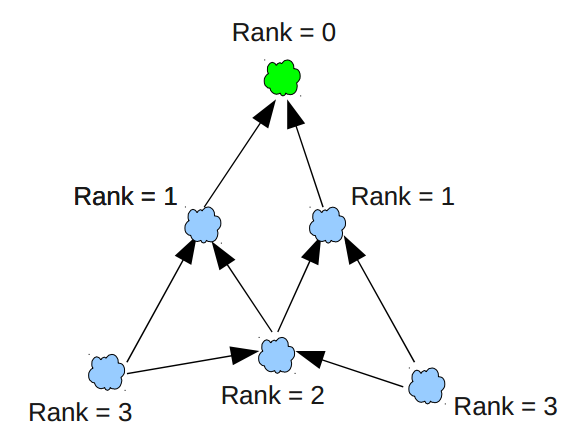
\includegraphics[width=0.6\textwidth]{fig/dodag.png}
		\caption{A DODAG}
		\label{Fig: DODAG}
	\end{figure*}
	
	We omit further details of the decision of a routing path as it is beyond the scope of this report but they are defined in \cite{rfc6550}. We explain the major RPL Messages in a 6LoWPAN network.
	
	\begin{description}[style=nextline]
		\item[\textbf{DAG Information Object (DIO) Message}]
		The DIO message contains the global information of a 6LoWPAN network. It is broadcasted by a node to its neighbours periodically for maintenance, or as a reply on request of a new joining node to provide enough information for the new one to join the network.
		\item[\textbf{DAG Information Solicitation (DIS) Message}]
		When a new node is booted, it broadcasts DIS messages probing an existing 6LoWPAN network. If the DIS message is received by any neighbour node that belong to a network, then a DIO message is replied providing the information to join the network.
		\item[\textbf{Destination Advertisement Object (DAO) Message}]
		DAO Message is sent by a child node to its precedents to propagate its routing information. The routing information is later used when another node tries to send a packet to this child node. The receiving parent can either store the routing information or forward it to an upper level parent depending on its capability.
	\end{description}
	
	\cite{rfc6550} also defined secure variants to these RPL Messages which provides authentication as well as confidentiality. However, they are not implemented on our platform and therefore we omit their details in this report.
\end{description}

\section{Transport Layer} \label{Sec: Transport Layer}
Transport Layer defines the interfaces that can be directly used by applications. To be more specifically, ports are defined to complement network addresses, allowing the kernel to direct application data to the correct procedure running on the host. Transport Layer protocols define also communication primitives to applications, such as reliability and stream/block wise data.

TCP and UDP are the most widely used Transport Layer protocols over Internet. TCP provides a reliable stream connection whilst UDP provides only unreliable datagram transmission. In case of WSN, UDP is generally preferable than TCP due to its low overhead and multicast support.

\subsection{UDP}

UDP is defined by \cite{rfc768}. The format of an UDP datagram is shown in \Cref{Fig: UDP Datagram Format}.

\begin{figure*}[h!]
	\center
	\begin{tabular}{ccccc}
		\multicolumn{4}{c}{\textit{UDP Header}}                                                                                                                & \textit{UDP Payload}         \\ \hline
		\multicolumn{1}{|c|}{2 (bytes)} & \multicolumn{1}{c|}{2}                & \multicolumn{1}{c|}{2}              & \multicolumn{1}{c|}{2}        & \multicolumn{1}{c|}{*}       \\ \hline
		\multicolumn{1}{|c|}{Source Port}        & \multicolumn{1}{c|}{Destination Port} & \multicolumn{1}{c|}{Payload Length} & \multicolumn{1}{c|}{Checksum} & \multicolumn{1}{c|}{Payload} \\ \hline
	\end{tabular}
	\caption{UDP Datagram Format}
	\label{Fig: UDP Datagram Format}
\end{figure*}

\begin{description}[style=nextline]
	\item[\textbf{Source and Destination Port}]
	Ports are the identifier of applications running on a host. Source and Destination Port semantically represent the sending and receiving procedure of application data respectively.
	\item[\textbf{Payload Length}]
	The length of Payload.
	\item[\textbf{Checksum}]
	Checksum of the datagram. The checksum is optional in \cite{rfc768} but is mandatory in 6LoWPAN.
	\item[\textbf{Payload}]
	This is the actual application data.
\end{description}

The UDP header consumes only 8 bytes. Data transmission using UDP is unreliable, i.e. the data might be lost, modified or arrived disordered. 

\section{Application Layer}
Application Layer represents the various applications. Other contexts may categorise some of the protocols differently, e.g. DTLS in \Cref{Subsec: DTLS} may be viewed as a security sub layer protocol in Transport Layer and CoAP in \Cref{Subsec: CoAP} can also be viewed as a Transport  Layer protocol since it defines reliable transmission primitives, etc.

For generality we describe two typical Application Layer protocols in this section that has been implemented on our platform, namely DTLS\cite{rfc6347} and CoAP\cite{rfc7252}. Applications can be built above these protocols.

\subsection{DTLS} \label{Subsec: DTLS}
DTLS\cite{rfc6347} stands for Datagram Transport Layer Security, the datagram variant of TLS. As of TLS, it provides end-to-end data confidentiality and authenticity. The main differences between DTLS and TLS are that:

\begin{itemize}
	\item DTLS builds on unreliable datagram communication, comparing to TLS which builds on reliable stream connection like TCP. In case of 6LoWPAN, DTLS is effectively built on UDP. DTLS implements a simple reliable transmission mechanism to exchange critical cryptographic materials during the handshake phase.
	\item Explicit sequence number and epoch values on each DTLS record. We explain more details in the following context.
	\item Invalid records no longer terminate the connection. Instead, in most of the cases errors are suppressed to the upper layer application.
	\item RC4 is disabled due to its stateful design,  as it is hard to synchronise two ends of the DTLS connection with UDP. \cite{DtlsCiphers} defines the available cipher suites in DTLS.
\end{itemize}

A DTLS packet is called a record. Its format is as depicted in \Cref{Fig: DTLS Record Format}.

\begin{figure*}[h!]
	\center
	\begin{tabular}{cccccc}
		\multicolumn{5}{c}{\textit{DTLS Header}}                                                                                                                                     & \textit{DTLS Encrypted Payload} \\ \hline
		\multicolumn{1}{|c|}{1 (byte)}     & \multicolumn{1}{c|}{2}                & \multicolumn{1}{c|}{2}     & \multicolumn{1}{c|}{6}               & \multicolumn{1}{c|}{2}      & \multicolumn{1}{c|}{*}          \\ \hline
		\multicolumn{1}{|c|}{Content Type} & \multicolumn{1}{c|}{Protocol Version} & \multicolumn{1}{c|}{Epoch} & \multicolumn{1}{c|}{Sequence Number} & \multicolumn{1}{c|}{Length} & \multicolumn{1}{c|}{Fragment}   \\ \hline
	\end{tabular}
	\caption{DTLS Record Format}
	\label{Fig: DTLS Record Format}
\end{figure*}

\begin{description}[style=nextline]
	\item[\textbf{Content Type}]
	Content Type is inherited from TLS. It indicates the type of this record. The value can either be:
	\begin{enumerate}
		\item CHANGE\_CIPHER\_SPEC($20$)
		\item ALERT($21$)
		\item HANDSHAKE($22$)
		\item APPLICATION\_DATA($23$)
	\end{enumerate}
	In cases of CHANGE\_CIPHER\_SPEC and HANDSHAKE, the relative sub protocols are invoked accordingly. In other cases the Fragment field is treated as an error code for ALERT record or ciphertext of application data for APPLICATION\_DATA.
	\item[\textbf{Protocol Version}]
	DTLS uses the complement of \{0xff, 0xff\} to indicate the version number. Since the implementation on our platform is for DTLS 1.2, this field is constantly \{0xfe, 0xfd\}.
	\item[\textbf{Epoch}]
	This field is increased by one for each cipher state change, such as an invocation of \\
	CHANGE\_CIPHER\_SPEC. This value is used as an index of cryptographic materials to be used, including algorithms, keys nonces nonces.
	\item[\textbf{Sequence Number}]
	This field is the sequence number of records, increased by one for each record.
	\item[\textbf{Length}]
	The length of Fragment.
	\item[\textbf{Fragment}]
	The content of Fragment depends on Content Type as explained above.
\end{description}

The DTLS on Contiki is implemented by a third party code, tinydtls-0.8.2\cite{tinydtls}. Its current version supports two ciphersuites, namely:
\begin{itemize}
	\item TLS\_ECDHE\footnote{Elliptic Curve Diffle-Hellman key Exchange}\_ECDSA\footnote{Elliptic Curve Digital Signature Algorithm}\_WITH\_AES\_128\_CCM\_8\cite{rfc7251}
	\item TLS\_PSK\footnote{Pre Shared Key}\_WITH\_AES\_128\_CCM\_8\cite{rfc6655}
\end{itemize}
Both cipher suites adopt the same AEAD scheme, AES\_128 with 8 bytes CBC-MAC in CCM mode, as their cryptographic primitives. Further details of the AEAD schemes are defined in \cite{rfc5116} and \cite{CCM}.

One thing to be noticed is that DTLS is not compatible with the multicast feature of IPv6 and UDP. The direct reason is the distribution of cryptographic materials poses a great difficulty in IoT applications. \cite{DtlsMulticast1} and \cite{DtlsMulticast2} discuss this topic in further details.

As of this project, we are mostly focused on the APPLICATION\_DATA records rather than the handshake process, as we consider the later to be performed independently from any upper layer application.

\subsection{CoAP} \label{Subsec: CoAP}
Constrained Application Protocol, CoAP, is a general application framework defined by \cite{rfc7252}. CoAP can be viewed as a variation of HTTP that is specifically designed to access or manipulate resources on IoT devices. The high level concept of CoAP is to make communication to sensor nodes behaves in a similar manner of accessing a web site. Generally speaking,
\begin{itemize}
	\item Typically the sensor node runs a CoAP server application registering its resources (sensors, actuators). The management node, operated by an user or higher level application, access the sensor node as a CoAP client. 
	%In cases where the sensor node can also be a CoAP client and requests operational information from the management node which in this case runs as a CoAP server.
	\item Similar to HTTP, CoAP uses a Request-Response application model. That is, the CoAP client actively sends a Request to CoAP server and the CoAP server passively replies with a Response.
\end{itemize}

We show an example of the execution of CoAP protocol in \Cref{Fig: An Example of CoAP}.
\begin{figure*}[h!]
	\center
	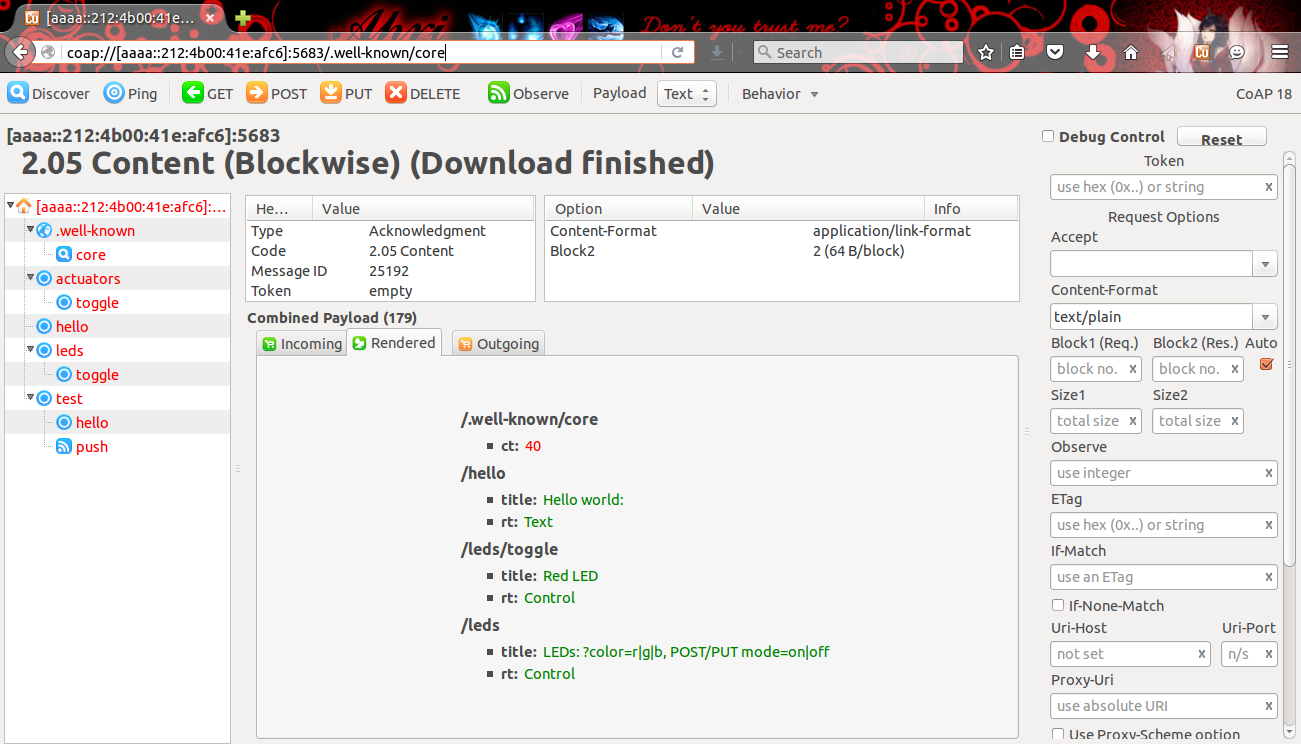
\includegraphics[width=1\textwidth]{fig/CoapExample.png}
	\caption{An Example of CoAP}
	\label{Fig: An Example of CoAP}
\end{figure*}

In the example of \Cref{Fig: An Example of CoAP}, the CoAP server is a CC2538 node registered with several resources listed in the tree view on the left, such as ‘’actuators’’, ‘’hello’’ and ‘’leds’’, etc. The CoAP client runs on a desktop through the Copper plugin\cite{Copper} of Firefox. As shown in \Cref{Fig: An Example of CoAP}, the CoAP framework has the following features:
\begin{itemize}
	\item A node in a 6LoWPAN network is represented by an URL. In \Cref{Fig: An Example of CoAP}, we can see at the address bar the resources of node is represented in a form of URL:\\
	\url{coap://[aaaa::212:4b00:41e:afc6]:5683/.well-known/core} \\
	This is exactly the same format of those URLs on Internet\cite{rfc3986}: \\
	 \{PROTOCOL :// ADDRESS : PORT / PATH \}.
	 \item Resources available on the node is organised in a tree structure, as shown in the tree view on the left in \Cref{Fig: An Example of CoAP}. These resources can be specified by the URL as shown in the address bar.
	 \item Similar to HTTP, four methods, namely GET, POST, PUT and DELETE, are defined to access and manipulate the resources on sensor nodes. In addition, the new option OBSERVE is defined for GET method to allows a CoAP server to actively push data to the CoAP client. We explain more details of these methods later in the context.
\end{itemize}

In addition, CoAP also provides a lightweight reliable transmission mechanism including fragmentation\cite{CoapBlock}; therefore some context uses CoAP as a reliable transmission protocol that is an alternative of TCP. For example, \cite{CoDTLS} proposes to use CoAP to perform the DTLS handshake instead of the built in retransmission mechanism of DTLS. CoAP also supports multicast messages as it is based on UDP, comparing to HTTP which is generally based on TCP and  hence supports only one to one communication.

\Cref{Fig: CoAP Message Format} describes the format of a CoAP message. The Token and Options uses a length-value representation. The length of Payload is not explicitly stated but is calculated by the payload length of upper layer protocol.
\begin{figure*}[h!]
	\center
	\begin{tabular}{|c|c|c|c|c|c|c|c|c|}
	\hline
	2 bits  & 2 bits & 4 bits       & 1 byte & 2 bytes   & * & *       & 1 byte    & *       \\ \hline
	Version & Type   & Token Length & Code   & Message ID & Token                 & Options & Payload Marker & Payload \\ \hline
	\end{tabular}
	\caption{CoAP Message Format}
	\label{Fig: CoAP Message Format}
\end{figure*}

\begin{description}[style=nextline]
	\item[\textbf{Version}]
	This is the version of CoAP. Currently this is constantly 0x01.
	\item[\textbf{Type}]
	Type field contains the transmission related information. There are four values defined:
	\begin{itemize}
		\item \textbf{Confirmable(0)}: The message must be confirmed by an acknowledgement, otherwise the sender will attempt to retransmit the message.
		\item \textbf{Non confirmable(1)}: The message does not need to be confirmed and thus the transmission is unreliable.
		\item \textbf{Acknowledgement(2)}: This value is set to inform the reception of a Confirmable(0) message. Piggyback, i.e. application data sent together within the same message, is allowed in CoAP acknowledgement. In some context this is abbreviated as ACK.
		\item \textbf{Reset(3)}: This value is similar to the RST flag in TCP which usually indicates a fatal error in connection and no further messages should be sent.
	\end{itemize}
	\item[\textbf{Token Length}]
	This field indicates the length of Token.
	\item[\textbf{Code}]
	Code indicates the class of content in this message. The higher 3 bits represents:
	\begin{itemize}
		\item \textbf{Request(0)}: Sent by client requesting operation on resources.
		\item \textbf{Success Response(2)}: A Response by server indicates a successful Request.
		\item \textbf{Client Error Response(4)}: A Response by server indicates an error in the Request. This can be resulted from syntax error in Request or the serve is not capable to process the Request.
		\item \textbf{Server Error Response(5)}: A Response by server indicates an error happened in the server. In this case, the Request is valid but the server failed due to some internal error.
	\end{itemize}
	The lower 5 bits indicates further details of the code.
	If the message is a Request, these bits indicates the method of this Request:
	\begin{description}[style=nextline]
		\item[\textbf{GET}] 
		The client requests to read a resource. Specifically when the OBSERVE option is set for a GET request, the resources can be pushed to the client  without further Requests\cite{rfc7641}.
		\item[\textbf{PUT}] 
		The client requests to write a resource to a value it provides.
		\item[\textbf{POST}] 
		The client requests to update a resource by a value it provides.
		\item[\textbf{DELETE}]
		 The client requests to remove a resource.
	\end{description}
	By definition, GET, PUT and DELETE are idempotent, i.e. execution of Request is stateless. However, the definitions above are only semantic and are not mandatory. Implementation could still violate the definitions, such as modifying the data on a GET Request.
	
	In case of a Response, the lower bits inherited the error codes in HTTP, as defined in \cite{rfc2616}.
	\item[\textbf{Message ID}]
	Message ID is the index of a message. It is mostly used in reliable transmission to match an acknowledgement with its original message.
	\item[\textbf{Token}]
	Token is an index for a Request-Response session. A Response is matched to a Request by Token. Notice that Message ID and Token are different indexes, since same Token might be reused for multiple messages due to fragmentations, or OBSERVE option, etc.
	\item[\textbf{Options}]
	Options are the arguments for a message similar to their counterpart in HTTP, such as URI, content format and size, etc. Different Options are based on Code. The detailed data structure and full list of Options is defined by \cite{rfc7252}.
	\item[\textbf{Payload Marker}]
	Payload Marker marks the end of Options. Any data followed should be treated as Payload.
	\item[\textbf{Payload}]
	Application data contained in this message. 
\end{description}

Based on the similarity between CoAP and HTTP, a CoAP message can be easily translated to a HTTP message and vice versa through a Cross-Protocol Proxy, as depicted in \cite{rfc7252}.

Erbium\cite{Erbium} project is the CoAP implementation on Contiki, described in \cite{ContikiCoap}. It implements the CoAP engine and defines an interface for developers to implement their own application over CoAP framework. 
%Simply speaking, what developers need to do to integrate their own code into the CoAP framework is simply register their own callback function to the CoAP server to handle the Requests to different resources.

\subsection{CoAPs} \label{Subsec: CoAPs}
CoAPs is the security version of CoAP which is a counterpart of HTTPS to HTTP. CoAPs adopts DTLS as the security measure. Any CoAP message should be encrypted as DTLS payload when using CoAPs. CoAPs is defined by \cite{rfc7252}. An overview of CoAPs meesage is shown in \Cref{Fig: CoAPs Message}.

\begin{figure*}[h!]
	\center
	\begin{tabular}{cc}
		\textit{}                                  & \textit{DTLS Encrypted Payload}            \\ \hline
		\multicolumn{1}{|c|}{\textit{DTLS Header}} & \multicolumn{1}{c|}{CoAP Message} \\ \hline
	\end{tabular}
	\caption{CoAPs Message}
	\label{Fig: CoAPs Message}
\end{figure*}

The current version of DTLS does not support the multicast feature of CoAP. The multicast alternation of DTLS proposed by \cite{DtlsMulticast1} and \cite{DtlsMulticast2} could be used to adapt CoAPs to multicast messages.

\cite{Lithe} proposes an integration of CoAP and DTLS with compressed headers. Unfortunately we have failed to adapt its source code to our platform. We have yet found any concrete CoAPs implementation on our platform.

\section{RIME Stack}
RIME Stack\cite{RIME} is a non-layered WSN communication framework proposed implemented in earlier version of Contiki. Instead using the layered structure as OSI model does, RIME Stack organises the communications of WSN in a way such that:
\begin{itemize}
	\item Each node is identified by a RIME address. In practice, the RIME address is directly derived from the hardware address.
	\item RIME Stack defines a set of abstracted communication primitives and arguments that can be directly invoked by the applications.
	\item The Chameleon architecture\cite{RIME} acts as a virtualisation layer that translates RIME Stack calls into MAC frames and vice versa.
\end{itemize}

Comparing to 6LoWPAN, RIME Stack is more flexible and efficient. However, since routing is solely implemented by upper layer application, RIME Stack is not adequate to fast application development in scaled applications with complicated communication models.

\section{Summary}
%Protocol suite
In \Cref{Chp: Building Blocks} we introduced a set of building blocks that could be use to build a secure WSN.  We introduced the protocol stack layer by layer within a simplified OSI model, as summarised in \Cref{Tbl: Summary of WSN Building Blocks}:

\begin{table*}[h!]
	\center
	\begin{tabular}{|c|c|c|}
		\hline
		\textit{\textbf{Layer}}                                                                         & \textbf{Protocol}           & \textbf{Alternatives}  \\ \hline
		\multirow{2}{*}{\textit{Application Layer}}                                                     & Optional: CoAP                        & \multirow{2}{*}{Lithe} \\ \cline{2-2}
		                                                                                                & Optional: DTLS              &                        \\ \hline
		\textit{Transport Layer}                                                                        & UDP                         & TCP                    \\ \hline
		\multirow{2}{*}{\textit{Network Layer}}                                                         & Optional: IPSec (not yet supported)             &                        \\ \cline{2-3} 
		                                                                                                & 6LoWPAN                     & ZigBee, RIME Stack          \\ \hline
		\multirow{2}{*}{\textit{\begin{tabular}[c]{@{}c@{}}Data Link Layer\\ (MAC Layer)\end{tabular}}} & Optional: 802.15.4 Security, ContikiMAC & TSCH                   \\ \cline{2-3} 
		                                                                                                & \multirow{2}{*}{802.15.4}   & \multirow{2}{*}{BLE}   \\ \cline{1-1}
		\textit{Physical Layer}                                                                         &                             &                        \\ \hline
	\end{tabular}
	\caption{Summary of WSN Building Blocks}
	\label{Tbl: Summary of WSN Building Blocks}
\end{table*}

This protocol suite we adopted is expected to be general, as both 802.15.4 standard and 6LoWPAN are widely supported by recent IoT devices and are suitable to general WSN applications. CoAP is used in Application Layer for its generality and interoperability. We built our experimental WSN using this protocol suite with Contiki\cite{Contiki}.

OpenWSN\cite{OpenWSN} can alternatively be used to build a WSN as it supports the same ‘’802.15.4 + 6LoWPAN + CoAP’’ protocol suite, except that it implements TSCH instead of ContikiMAC. In addition, other systems and protocols could also be used, such as BLE\cite{BLE} in Physical and MAC Layer and ZigBee for Network Layer, etc. We leave the research on other platforms as future work.